\documentclass{article}
\usepackage{amsmath}
\usepackage{amssymb}
\usepackage{amscd}

\usepackage{biblatex}
\addbibresource{bibliography.bib}

\usepackage{graphicx}
\graphicspath{ {./images/} }

\usepackage{amsthm}
\theoremstyle{definition}
\newtheorem{definition}{Definition}[section]
\newtheorem{theorem}{Theorem}[section]


\title{Neural network knowledge distillation in tensor networks}
\author{Dereck Piché}
\date{\today}
\theoremstyle{definition}


\begin{document}
\maketitle

\begin{abstract}
\end{abstract}

\section{Introduction}



\section{Knowledge Distillation}
Knowledge Distillation is a machine learning practice which involves
taking a trained model and using its parameters to train another one.
The already trained model is referred to as the "teacher", and 
the model in which his "knowledge" is to be distilled is referred to as
the "student". While this is a relatively novel technique, there are 
already several distinct approaches introduced by researchers.
In this project, we used two of these approaches. Our inspiration for the distillation 
methodology was found in a a 2021 survey which resumed the emerging 
practice \cite{Gou_2021}.

\subsection{Response-Based Knowledge Distillation}
The first approach we used was \emph{Response-Based Knowledge Distillation}. The idea of this approach is to stimulate the teacher and the student with some input and to try to minimise a certain loss function with respect to the teacher and student outputs. For classification tasks, it is recommended to use the Kullback-Leibler divergence loss as our loss function. 
\begin{equation}
    KL(P, Q) = \frac{1}{n} \sum_i^n Q \frac{log_e(Q)}{log_e(P)}
\end{equation}
Here, $Q$ is the distribution we are aiming for and $P$ is the one we have.

The reason is quite simple. Since it's a classification task, it is expected that the teacher and student will, given an input, return a probability distribution for each class. As is currently common, we used the softmax function on the logits of the student and the teacher in order to obtain probability distributions corresponding to the classes. 

\begin{equation}
    softmax(v_i) = \frac{e^{v_i}}{\sum_{j}{e^{v_j}}}
\end{equation}

Now, it would be logical to use a function aimed at measuring the difference between two probability distributions as our loss function. This is exactly what the Kullback-Leibler divergence is for.

\subsection{Layer-based approach}
The survey on Knowledge Distillation coined the term {\it Layer-based approach}.
Deep learning models work in layers of feature maps. It is hypothesized that
these different layers represent different layers of abstraction in the internal
representation of their input. If we simply use the Response-Based approach, it could prove difficult for gradient descent otpimization to find these usefull representation without a bit of help. This layer-based approach, as you might have guessed, aims to do precisely that. If our student model has some form of composition, we can train the parts separately. Thus, if an intermediate layer of the teacher $l$ were particularly useful, we could train a certain part of the student on the layer $l$ before proceding with the Response-Based approach.



\section{Tensor Networks}
Tensor Networks are mathematical objects which were created by physicists in order to help the modelisation of quantum phenomena.
In 2017, researchers form TODO add the brilliant idea of using these networks as machine learning models.
In order to make this report as self-contained as possible, we decided to provide a short explanation of what they are.
Some confusion can be avoided by mentionning that the expression \emph{Tensor Networks} refers, in the scientific community, to both a series of methods and a notational system.

\subsection{Tensors}
Before explaining these two, we shall disambiguate the meaning of "tensor". 
In this report (and very often in the context of machine learning), we use the word "tensor" to refer to the mathematical arrays of arbitrary indices. 
Here, the number of indices is called the "order" of the tensor, meaning that vectors are simply tensors of order $1$ and matrices tensors of order $2$. 

\subsection{Contraction}
At the heart of tensor networks is the {\it contraction} operation.
Tensor Networks are used to compute a larger network by "contracting" several
smaller tensors over chosen indices. A "contraction" is simply an operation 
where we sum over indices. For example, the contraction of $A_{ijk}$ and 
$B_{ijk}$ on index $j$ will produce the tensor $C_{ik} = \sum_{j} A_{ijk} B_{ijk}$.
Evidently, the two indices present in a contraction must be of the same size.

\subsection{Tensor Networks as a graphical system of notation}
The principal motivation behind the creation of Tensor Networks to compute or approximate large tensors {\it contracting} several smaller tensors over chosen indices. 
This is all well and good until our conventional summation notation begins overclocking our primal brains.
So, in order to make the manipulation of these network of tensors, mathematicians created a notational system. 
Tensors are represented as nodes where each vertex connected to the node represents one of the tensor's indices. 
If a vertex connects two nodes, it means that the indices shall be contracted in order to produce the post-contraction tensor. 
It should be evident that by the definitions above, no node (tensor) is completely isolated in a tensor network, as it would be completely purposeless. 
The shape of the post-contraction tensor can be easily visually identified, since it is found in the unconnected vertices.
A simple tensor network can be found in figure \ref{fig:tensor_net}.

\subsection{Tensor Network Methods}
The term {\it Tensor Network Methods} is used to refer to, you guessed it, the methods.
There are several architectures of Tensor Networks that are frequently used, such as the {\it Matrix Product State (MPS)}, the {\it Tenso}.
There are many ways of transforming a Tensor into a contraction of smallers tensors. 
With time, some particular ways became popular for their properties. 
Some are faster to compute, some are clearer, some are easier to train in a machine learning context. 
One of these recurring architectures, the Matrix Product State, is at the core of the research done by the author.
Not only is there multiple valid ways of setting up the network for contractions, there are also different ways of performing the contraction.
In Tensor Networks, the order of contraction affects the computationnal complexity of the whole process!
All of these kinds of concepts are referred to by the expression \emph{Tensor Network Methods}.


\begin{figure}[h]
\centering
\caption{Simple tensor network illustrating the notation.}
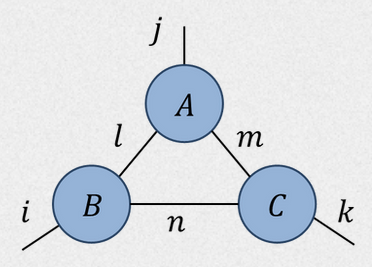
\includegraphics[width=0.5\textwidth]{images/2023-03-21-10-22-39.png}
\label{fig:tensor_net}
\end{figure}

\section{Creating the $\Upsilon$ function}
In this report, we used the MPS tensor network to approximate a particular parameterizable function.
{\bf Troughout this report, the parameterizable function we are approximating with the MPS will be denoted by $\Upsilon$. }
We found it clearer to explain the $\Upsilon$ function we are approximating before introducing the MPS tensor network, as we can explain it trough its use.
Now, enough talking (or rather, writing?), let's create the $\Upsilon$ function!

\subsection{Feature tensor $\Phi(x)$}
Consider an input vector $x \in R^d$. Let $\phi : R \mapsto R^{d_{\phi}}$ be a function which creates a feature map vector $\phi(\lambda)$ from its input $\lambda$.  We shall form the vector $\Phi(x)$ by taking the Kronecker product of the feature map $\phi(x_i)$ of every element of the input vector $x$.
\begin{equation}
    \Phi(x) = \phi(x_1) \otimes  \phi(x_2) 
                \otimes (\dots) \phi(x_d)
\end{equation}
Here, the symbol $\otimes$ represents the Kronecker Product. The Kronecker Product is an extremely generalisable operation that can be applied to a pair of tensors of arbitrary order. In this project, we use the Kronecker Product exclusively on vectors. Here is a simple example that illustrates what the kronecker product does for simple vectors of integers.
\[
\begin{bmatrix}
    9 \\ 4
\end{bmatrix}
\otimes
\begin{bmatrix}
    6 \\ 8
\end{bmatrix}
\otimes
\begin{bmatrix}
    7 \\ 3
\end{bmatrix}
=
\begin{bmatrix}
    54 \\ 72 \\ 24 \\ 32
\end{bmatrix}
\otimes
\begin{bmatrix}
    7 \\ 3
\end{bmatrix}
=
\begin{bmatrix}
    378 \\ 162\\ 504 \\216\\ 168\\ 72\\ 224\\ 96
\end{bmatrix}
\]
The element $i$ of the first operand vector becomes itself multiplied by the second operand vector. Here's a slightly more abstract example:
\[
    \begin{bmatrix}
        v_1 \\ v_2
    \end{bmatrix}
    \otimes
    \begin{bmatrix}
        u_1 \\ u_2
    \end{bmatrix}
    =
    \begin{bmatrix}
        u_1 v_1 \\ u_2 v_1 \\ u_1v_2 \\ u_2v_2
    \end{bmatrix}
\]
Thus, if we perform a Kronecker Product on $n$ vectors, it will produce a vector such that every of it's element is a multiplication of $n$ elements, each one from a different vector. We can thus interpret $\Phi(x)$ as being a feature space vector which \emph{captures the multiplicative interaction of the elements of the $\phi(x_i)$ feature maps}.



\subsection{The multilinear feature map}
Now, which feature map $\phi$ shall we pick in order to construct $\Phi$?
Well, normally, this would be up to you, but in this project we deal with the particular feature map
\begin{equation}
    \phi_{ml}(\lambda) = 
    \begin{bmatrix}
        1 \\
        \lambda
    \end{bmatrix}
\end{equation}
As the name of the subsection suggests, we call this particular feature map the \emph{multilinear feature map}.
But why do we call it that?
We call it that because, amazingly, when we use this feature map, the elements of $\Phi$ form a basis space of the multilinear functions on the elements of the vector $x$.
Understanding this statement without a bit of context and help is a tall order. Let's deconstruct it.
First, what is a multilinear function?


\subsection{Linear Combinations}
When we introduced $\Upsilon$, we said it was a parameterizable function.
However, as of yet, everything described about the function as been deterministic and fully specified.
Tbus, it is time to introduce the parameters. 
Now, the question is how do we use $\Phi(x)$, how does it become useful? 
Well, it becomes useful when we take a linear map of its elements. Let our $\Phi(x)$ be an 
arbitrarily shaped tensor of $d_{\Phi}$ dimensions. The final form of our 
function $f(x)$ will be
\begin{equation} \label{eq:model}
    f(x) = \sum_{i}^{d_{\Phi}} \theta_i [\Phi(x)]_i
\end{equation}
Now, we have a function that can, under some choice of transformation
$\phi$, become extremely expressive. For our particular local feature map 
$\phi^*$, it can represent any multililinear function  of the input vector $x$. 
We shall represent linear combinations of $\Phi(x)$ by $T\Phi(x)$.

\section{Using The Matrix Product State Tensor Network}

In this project, we used the {\it Matrix Product State} (MPS) tensor network to 
approximate the function $T  \Phi(x)$. Here, this function is computed by contracting 
a Tensor Network. Before the contraction, some of the elements of the tensors in the 
tensor network are set by applying the mapping $\phi^*(x)$.

\subsection{Building the model using a single MPS}
As proposed in the paper \cite{stoudenmire2017supervised}, we are going to use 
a particular Tensor Network Method in order to reproduce a model of the form \ref{eq:model}.
Before going over the use of MPS, let's think of a way to use tensors and contraction to 
learn a model of a function $f: R_d \mapsto R_q$. First, we create a tensor of the form $T^{o_1 o_2 (\dots) o_d i}$, 
where, each $o$ is of dimension $2$ and $i$ is of dimension $q$ (the dimension of the output of $f$). Then, if we apply a contraction 
between every $o_i$ and its corresponding vector $\begin{bmatrix}1 \\x_i\end{bmatrix}$, we obtain
a function $m: R_d \mapsto R_q$. Our model $m$ can learn $f$ by adjusting the parameters of the tensor 
$T$ by supervised learning.

\paragraph{} ${}$ \\
The problem is that as of now, the tensor $T$ has $2^{d}$ elements. In order to 
reduce the size of $T$, we can approximate it by using a decomposition called 
the \emph{Matrix Product State}.
\begin{equation} \label{eq:mps_approx}
T^{o_1 o_2 (\dots) o_d} \approx T_{MPS} = 
\sum_{ \{ b_1,b_2,(\dots), b_d \}} t^{o_1}_{b_1} t^{o_2}_{b_1, b_2} t^{o_3}_{b_2 b_3} \dots  t^{o_d}_{ b_{d-1} } 
\end{equation}

Here, the complexity of the MPS is determined by the \emph{bond dimension} of its tensors.
The \emph{bond dimension} of $T_{MPS}$ is the dimension of the contracted indices of the network.
In equation \ref{eq:mps_approx}, it would be the dimension of the $b$ indices.

Now, our goal is rather to use the MPS to perform a certain computation, not compress tensors. 

In order to do this, we will contract every index of the tensor $B$.
TODO: add number of parameters of MPS and how it grows with respect to size

\subsection{Composition of MPS}
As mentionned before, taking a linear map of  tensor product of the local feature map 
$ \begin{bmatrix} 1 \\ x \end{bmatrix} $ amounts to producing a multilinear function of $x$.

Since our MPS model can only approximate this function, it means that its expressivity
will be somewhat limited. For example, it could never express the function $f(X) = x_1x_2^2$.

A pretty obvious solution for this problem is to add another layer by feeding to ouputs of 
our MPS model into a second one.

Instead of looking at the expressivity of this composition directly, we will analyse 
the expressivity of the functions that the MPS models are trying to approximate. This 
will give us a good idea of how expressive this composition can be. Also, from now on,
this composition will be refered to as \emph{2-MPS}.

The 2-MPS model approximates a function of the form.
\[  
    g' \circ f \circ g \circ f (x)
\]

In the following subsection, we will prove that this composed function can express
any multivariate polynomial function of degree $z$.

\subsubsection{Proof of expressivity}

\begin{definition}[A $\psi$ function]
    A multilinear polynomial is a function $f: R^n \mapsto R$ of the form
    A $\psi$ function is a function of the form
    \[  g' \circ f \circ g \circ f (x) \],
    where $f$ is a function that returns a basis of a multililinear function and 
    $g'$ and $g$ are arbitrary linear maps.
\end{definition}


\begin{definition}[Multilinear polynomial]
    A multilinear polynomial is a function $f: R^n \mapsto R$ of the form
    \begin{equation}
        f(x) = T \cdot \left( 
            \begin{bmatrix} 1 \\ x_1 \end{bmatrix} \otimes 
            \begin{bmatrix} 1 \\ x_2 \end{bmatrix} \otimes 
            \dots \otimes 
            \begin{bmatrix} 1 \\ x_d \end{bmatrix}
        \right)
    \end{equation}
    Where $T \in R^{p \times R^n }$. In other words, a multilinear polynomial is a polynomial that is linear if  $\forall x_i$ then the polynomial is linear if we fix every variable except $x_i$.
\end{definition}

\begin{definition}[$v_i$-variate]
Function of the variables of the vector $v$. (Each element of $v$ is considered as a variable).
\end{definition}


\begin{theorem}
    Any polynomial function $\Gamma: R^d \mapsto R$ of degree $z$ can be expressed as
    a $psi$ function by choosing particular $g'$ and $g$ maps.
\end{theorem}

\begin{proof}
Let the function $g$ in a $\psi$ function be defined such that

\begin{equation}
    g(f(x))
    = 
    \begin{bmatrix}
        \textit{repeated $z$ times} 
        \begin{cases}
            x_1 &  \\
            (\dots) & \\
            x_1 & 
        \end{cases} \\
        \textit{repeated $z$ times} 

        \begin{cases}
            x_2 &  \\
            (\dots) & \\
            x_2 & 
        \end{cases} \\
        (\dots) \\
        \textit{repeated $z$ times} 
        \begin{cases}
            x_n &  \\
            (\dots) & \\
            x_n & 
        \end{cases} \\
    \end{bmatrix}
\end{equation}
We can rewrite this vector as 

\begin{equation} \label{lambda}
    g(f(x))
    = 
    \begin{bmatrix}
        \varepsilon_{1, 1} \\
        (\dots) \\
        \varepsilon_{1, z} \\
        \varepsilon_{2, 1} \\
        (\dots) \\
        \varepsilon_{2, z} \\
        (\dots) \\
        \varepsilon_{d, z} 
    \end{bmatrix}
    = \lambda
\end{equation}

Let $Z$ be the space of $x_i$-variate polynomial functions 
of degree $\leq z$. By definition, every monomial of $\zeta \in Z$ is of the form
\begin{equation}
    x_{1}^{k_1}x_{2}^{k_2}(\dots)x_{d}^{k_d}
\end{equation}
, where $\sum k_i \leq z$. \\
However, for every set $\{k_1, k_2, (\dots), k_d\}$ meeting this condition,
we can rewrite the monomial as
\begin{equation}
    \left( \prod_{i_1=1}^{k_1}\varepsilon_{1, i_1} \right)
    \left( \prod_{i_2=1}^{k_2}\varepsilon_{2, i_2} \right)
    \left( \dots \right)
    \left( \prod_{i_d=1}^{k_d}\varepsilon_{d, i_d} \right)
\end{equation}
by using the elements of $\lambda$ from equation \eqref{lambda}.

However, we can clearly see that this term is a multilinear 
monomial of the variables in $\lambda$. This implies that
$f(\lambda*)$ returns a basis-vector of $x_i$-variate polynomial 
function of degree $\leq z$.

In other words, 
\begin{equation}
    \xi \left( x, \Theta \right) =
        M
        \left(
            f
            \left(
                M
                \left(
                    f
                    \left(
                        x 
                    \right),
                    \Theta^*
                \right)
            \right),
            \Theta
        \right)
\end{equation}
can express any $x_i$-variate polynomial function of degree $\leq z$ under
fixed $\Theta$.

This process can be visualised as 
\begin{equation} \label{composition_graph}
    \begin{CD}
        @. X \in R^d 
        @>f>> Y_1 \in R^{2^d}
        @>g>> Y_2 \in R^{zd} 
        @>f>> Y_3 \in R^{2^{zd}}
        @>g'>> Y_4 \in R
    \end{CD}
\end{equation}

\end{proof}

\subsection{Patching of MPS (experimental)}






\section{Methodology}
The experiments done for the projet were programmed using Python and the wonderful deep learning library Pytorch, created by Meta.
Unfortunately, Pytorch does not provide any tools to train and build Tensor Networks. 
Luckily for us, Jacob Miller, created a library \cite{torchmps} built on top of Pytorch that provides the tools to build and train MPS Tensor Networks. 

TODO: mention custom feature map in forked code

\paragraph{Learning rate} ${}$ \\
We used the very standard learning rate of $1e-4$. This is the proposed learning 
rate in the code of \cite{torchmps}.

\paragraph{Model size} ${}$ \\

\paragraph{Approach to the results}
As a matter of scientific integrity, we have chosen to show the 
results even if they are heavily disappointing. Not doing so 
can result in certain statistical biases which can be avoided.

Learning rate for neural network: 0.01
Learning rate for MPS: 1e-3 = 0.001
Nb of normal epochs: 25
Nb of gaussian epochs: 5


\section{Results}
\begin{tabular}{ | c | c | c | c |  }
\hline 
Bond Dimensions & MPS & FC to MPS & CNN to MPS \\ 
\hline
10 & $0.897 \pm 1.34 \times 10^{-4}$  & $0.541 \pm 9.50 \times 10^{-5}$ & $0.906 \pm 8.49 \times 10^{-5}$ \\
20 & $0.911 \pm 12.90 \times 10^{-4}$ & $0.550 \pm 9.32 \times 10^{-5}$ & $0.924 \pm 6.77 \times 10^{-5}$ \\ 
40 & $0.914 \pm 8.15 \times 10^{-5}$ & $0.556 \pm 5.99 \times 10^{-5}$ & $0.941 \pm 4.38 \times 10^{-5}$ \\
\hline
\end{tabular}

\section{Results}
\begin{tabular}{| c | c | c | }
\hline 
Bond Dimensions & 2-MPS & NN to 2-MPS \\ 
\hline
10 & $0.897 \pm 1.34 \times 10^{-4}$ & $0.897 \pm 1.34 \times 10^{-4}$ \\
20 & $0.897 \pm 1.34 \times 10^{-4}$ & $0.897 \pm 1.34 \times 10^{-4}$ \\
40 & $0.897 \pm 1.34 \times 10^{-4}$ & $0.897 \pm 1.34 \times 10^{-4}$ \\
\hline
\end{tabular}

\section{Analysis}



\section{Conclusion}



\subsection{Further Exploration}
TODO talk about capturing locality in the mappings
TODO talk about capturing locality in general with tensors

\printbibliography

\end{document}




































Person 1: *waiving vigorously
    HELLO CAN YOU SEE ME!
    HEYYY! 

Person 2:
    For the last time, they can't see you... 
    YOU'RE OUTSIDE THE DOCUMENT DELIMITERS!

Person 1: 
    I feel so alone... 

Person 2: 
    Bro I'm here...